\documentclass[10pt,letterpaper]{article}
\usepackage[margin=0.68in,headheight=14pt,footskip=22pt]{geometry}
\usepackage[T1]{fontenc}
\usepackage{lmodern}
\usepackage{microtype}
\usepackage{amsmath,amssymb,booktabs,array,graphicx}
\usepackage{xcolor}
\usepackage[hidelinks]{hyperref}
\usepackage{fancyhdr}
\definecolor{ink}{HTML}{172033}
\definecolor{blue}{HTML}{24598C}
\hypersetup{pdftitle={Sampling Efficiency and Geometric Sensitivity in Cardiff: A Controlled Porto Inference Study},pdfauthor={Zhijing Wu},pdfsubject={Independent controlled inference pilot; not a full benchmark reproduction}}
\pagestyle{fancy}
\fancyhf{}
\fancyhead[L]{\small\color{blue}CARDIFF \quad / \quad INDEPENDENT TECHNICAL NOTE}
\fancyhead[R]{\small 14 October 2026}
\fancyfoot[C]{\small\thepage\ / 2}
\renewcommand{\headrulewidth}{0.3pt}
\setlength{\parindent}{0pt}
\setlength{\parskip}{3.5pt}
\setlength{\tabcolsep}{7pt}
\newcommand{\topic}[1]{\vspace{3pt}{\color{blue}\bfseries #1}\par\vspace{-2pt}}
\newcommand{\code}[1]{\texttt{\small #1}}
\begin{document}
\color{ink}
\begin{center}
{\fontsize{16}{19}\selectfont\bfseries Sampling Efficiency and Geometric Sensitivity in Cardiff:\par
A Controlled Porto Inference Study}\par
\vspace{5pt}
{\normalsize\bfseries Zhijing Wu}\par
{\small Sichuan University \quad|\quad \href{mailto:zhijingwu.cs@gmail.com}{zhijingwu.cs@gmail.com}}\par
{\small \url{https://zhijingwu.github.io}}\par\vspace{4pt}
{\small Released Porto checkpoints \quad|\quad 64 conditions $\times$ 3 seeds \quad|\quad Inference only}
\end{center}
\vspace{-3pt}
\textbf{Finding.} Holding generated segment-level latents fixed, increasing the GPS sampling interval from 20 to 50 gave a median paired-batch speedup of \textbf{2.503$\times$} (conditional 95\% bootstrap interval: \textbf{2.432--2.692$\times$}). The pilot passed all eight frozen point-estimate criteria. Core length and step-distance summaries were close, while the turning-angle tail changed. These are execution and geometric diagnostics, not evidence of road validity or improved physical realism.

\topic{Framework and independent question}
Cardiff [1] first compresses discrete road-segment sequences with an autoencoder, generates segment latents with diffusion, and then generates continuous GPS coordinates with a latent-conditioned diffusion model. Our question was narrower than its benchmark: \emph{how do GPS-stage sampling cost and descriptive geometry change when its first-stage generated conditions are kept fixed?} No model training or new sampling algorithm was introduced.

\topic{Verified assets and controlled protocol}
The official repository [2] was pinned to revision
\code{1138b1ef0646c18e878608a848dafca018b8a888}.
Original Porto diffusion state dictionaries loaded with \code{weights\_only=True} and \code{strict=True}; no keys were missing or unexpected. Formats were inspected before loading. Unchanged SHA-256 values:
{\scriptsize\ttfamily
\par denoiser0: 09d66ff627e173de6fb75c9cfe0ae130c12a814c8e75d2ce02696ff1f2fba070
\par denoiser1: c6bda8e0a67b969d055f37420e527b70e390fecf35f489994568342cac45c02d
\par}
The first 64 valid attribute rows, in original order, were used with seeds 0, 1 and 2. Stage 1 latents were generated once per seed at interval 20, cached and reused in both GPS arms with identical attributes. The eight-condition smoke test returned latents $(8,32,128)$ and GPS $(8,2,64)$.

Eight-row batches alternated timing order and restored the same pre-call RNG state per pair; batches advanced from the interval-20 post-call state. CUDA-synchronized timings excluded setup, writing and Stage 1. The repeatability control matched exactly (maximum error 0). Effective $\eta=1$, original conditioning and FP32 were preserved. Hardware: 24 GB RTX 3090; Python 3.11.2, PyTorch 2.5.1+cu124 (versions differ from the author's recipe).

\topic{Measured GPS results: 192 trajectories per interval}
\begin{center}
\small
\begin{tabular}{@{}lrr@{}}
\toprule
Diagnostic & Interval 20 & Interval 50\\
\midrule
Total GPS wall time (s) & 41.797 & 16.702\\
Time per trajectory (ms) & 217.693 & 86.992\\
Finite-coordinate fraction & 1.000 & 1.000\\
Points outside preprocessing box & 2/12,288 & 0/12,288\\
Median cumulative geodesic length (m) & 3394.026 & 3377.722\\
Median consecutive-point distance (m) & 49.072 & 49.153\\
Pooled p95 consecutive distance (m) & 163.048 & 162.193\\
Pooled p95 unsigned turning angle ($^\circ$) & 62.224 & 54.180\\
\bottomrule
\end{tabular}
\end{center}
\vspace{-5pt}
Lengths use WGS84 geodesics and the original longitude/latitude denormalization:
mean $[-8.619011,41.15872626]$, standard deviation $[0.02382058,0.01060059]$.
Turns use a local equirectangular projection. Region containment is not a road-validity metric.

\newpage
\begin{center}
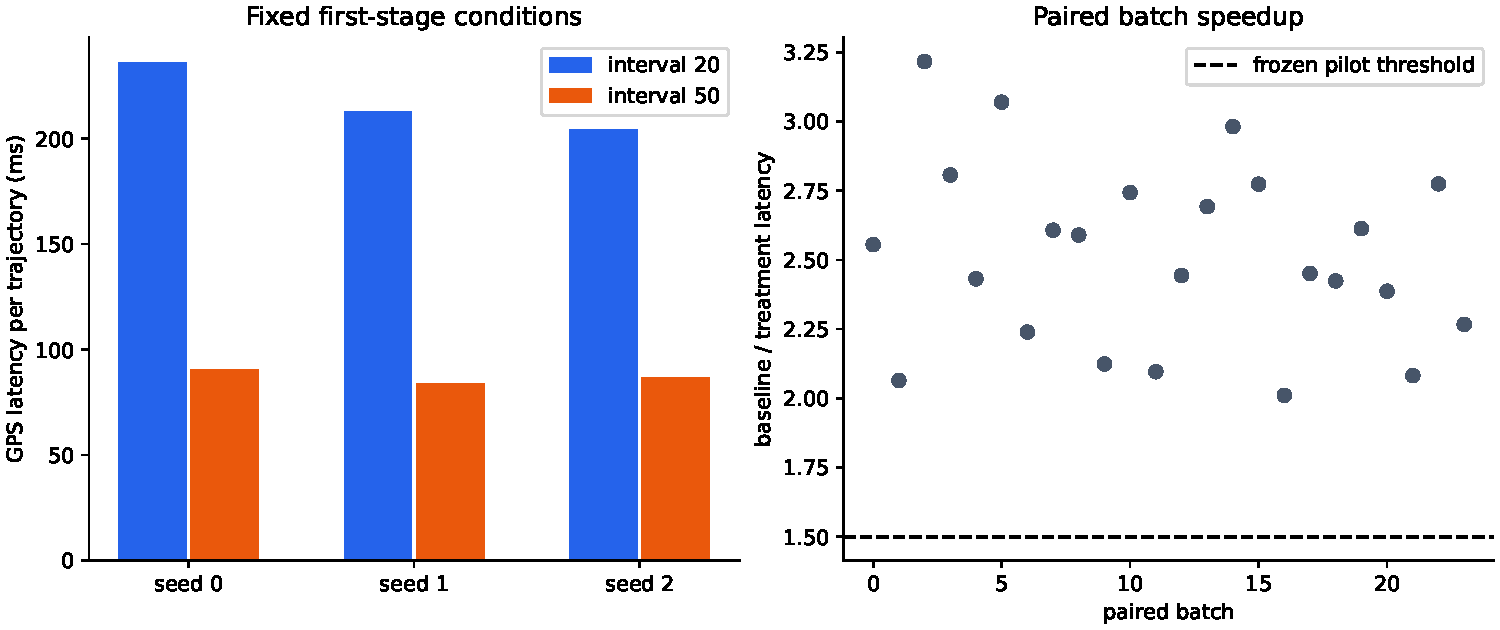
\includegraphics[width=0.94\linewidth]{figures/sampling_efficiency.pdf}
\end{center}
\vspace{-8pt}
{\small\textbf{Figure 1.} Preserved pilot figure: GPS latency by seed and 24 paired-batch speedups. Stage 1 was fixed within each pair. The dashed line is the frozen $1.5\times$ speedup criterion. No new model outputs or figure data were generated for this note.}

\topic{Uncertainty and exploratory sensitivity}
The median-length ratio (50/20) was 0.99520, conditional 95\% interval [0.94165,1.05557]; the pooled p95 step-distance ratio was 0.99475 [0.94610,1.02560]. Both point estimates passed the frozen $\pm10\%$ margins. All three seeds passed the core geometric margins, although effect directions varied.

The turning p95 ratio was \textbf{0.87072} [0.80529,0.92407], a roughly 12.9\% reduction. This is \textbf{exploratory}: no turning threshold was frozen, and a smaller angle is not established as better. A retained example also changes path shape. Aggregate agreement does not imply identical paths.

Geometry intervals use 2,000 paired attribute-ID resamples retaining all three seeds; timing intervals resample eight batch positions retaining the three seeds. These descriptive intervals are conditional on the ordered subset and RNG coupling. They are not population equivalence tests; only three seeds were studied.

\topic{What the RNG pairing controls}
The original wrapper sets $\eta=1$. Interval 20 uses 50 transitions from timestep 980; interval 50 uses 20 from 950. Restoring RNG states shares the unused latent Gaussian, initial GPS Gaussian and transition-noise prefix \emph{by draw index}. Those vectors enter different timesteps and coefficients; common timesteps generally use different draw indices. The comparison therefore combines stochastic schedule effects under one coupling and does not isolate deterministic discretization error.

\topic{Clean inference conditioning is intentional}
Paper section 3.5.2 prescribes generated latents without noise augmentation at inference, despite augmented training conditions. The helper computes but discards a noisy latent and uses auxiliary noise time 200; the meaning of that convention remains unconfirmed. Original behavior was retained. This is not a conditioning-noise ablation.

\topic{Limits and a proposed next question}
Cardiff already studies interval efficiency on Singapore [1, section 4.2.3]. This independent Porto pilot introduces no new interval method and does not reproduce benchmark scores. No matching road graph, decoded routes, checkpoint-matched held-out real reference, physical time model or privacy test was evaluated. Attribute split provenance is unknown; box containment and GPS geometry do not establish road validity.

\emph{Does faster GPS sampling preserve alignment with the same fixed segment-level road condition?} That question requires compatible decoder weights, the original segment-to-geometry mapping, independent held-out controls, asset permissions and a separately approved protocol. Road-alignment work is \textbf{proposed and has not been executed}.

\vspace{3pt}
{\footnotesize
\textbf{References and provenance}\par
[1] Baoshen Guo, Zhiqing Hong, Junyi Li, Shenhao Wang and Jinhua Zhao. \emph{Leveraging the Spatial Hierarchy: Coarse-to-fine Trajectory Generation via Cascaded Hybrid Diffusion}. arXiv:2507.13366v1 (2025).
\href{https://arxiv.org/abs/2507.13366v1}{arxiv.org/abs/2507.13366v1}.\par
[2] \emph{Cardiff}, official code and Porto release.
\href{https://github.com/urban-mobility-generation/Cardiff/tree/1138b1ef0646c18e878608a848dafca018b8a888}{github.com/urban-mobility-generation/Cardiff}, revision above.\par
Evidence and summary replay: \url{https://github.com/ZhijingWu/cardiff-sampling-geometry-audit}. Raw arrays and model weights are excluded. Independent study; no affiliation with or endorsement by the Cardiff authors.
}
\end{document}
